% Chapter 1

\chapter{Background} % Main chapter title

\label{Chapter1} % For referencing the chapter elsewhere, use \ref{Chapter1} 

%----------------------------------------------------------------------------------------

% Define some commands to keep the formatting separated from the content 
\newcommand{\keyword}[1]{\textbf{#1}}
\newcommand{\tabhead}[1]{\textbf{#1}}
\newcommand{\code}[1]{\texttt{#1}}
\newcommand{\file}[1]{\texttt{\bfseries#1}}
\newcommand{\option}[1]{\texttt{\itshape#1}}

%----------------------------------------------------------------------------------------

\section{Introduction}
	The idea for this independent study came from multiple conversations by the authors regarding the lack of a parallel or cluster computing course at the university. Subsequently, we have realized the importance of large scale processing in the age of big data. Understanding and analyzing big sets of data is a necessity in an age where almost all electronic devices (large and small) are connected to a network and feeding in trillions of data points per second. 
	
	We decided to utilize a set of Raspberry Pi computers as a small-scale example of a cluster computing platform. Initially, we thought that utilizing commodity hardware such as servers for our cluster would be the way to go. Unfortunately, we do not have access to such hardware, but after further research, we concluded that the Raspberry Pi would be sufficient to demonstrate concepts in parallel and cluster computing. 
	

%----------------------------------------------------------------------------------------

\section{Raspberry Pi }

	The Raspberry Pi is a low-cost, single-board computer that is capable of running light-weight GNU/Linux operating systems such as Raspbian. The Raspberry Pi utilizes the system on a chip (SoC) architecture in order to integrate components of the computer such as the microprocessor, graphics processing unit, and WiFi device. The Raspberry Pi is fairly easy to configure as there is a large, open-source community willing to help with setup issues. Additionally, the Raspberry Pi Foundation has put in a lot of effort to provide detailed and up-to-date documentation.

\subsection{ARM Architecture}

	The Raspberry Pi central processing unit utilizes the ARM Architecture developed by the ARM Holdings. The ARM architecture paradigm is extremely relevant as there have been over 100 billion devices produced (as of 2017) that utilize the ARM instructuction set architecture. Most handheld devices including iPads and gaming consoles utilize ARM cores.
	
	ARM, also known as Advanced RISC (Reduced Instruction Set Computing) Machine requires less transistors than x86 processors (usually found in personal computers) which make it an attractive candidate for embedded systems seeking to lower costs and energy consumption on devices. The ARM architecture supported only a core-bit width of 32, but the newest version of ARM, ARMv8 now supports both 32 and 64 bits as of 2011. Note, the Raspberry Pi utilizes ARMv7. ARMv7 adheres to the load/store architecture which separates instructions into memory access and ALU (Arithmetic Logic Unit) operations. Memory access is simply the process of transfering data from the memory to registers. ALU operations consist of the actual operations on the loaded memory. 

\subsection{Raspberry Pi 3}
	The Raspberry Pi 3 Model B consists of a quad-core 64-bit CPU with one gigabyte of RAM in the system on a chip configuration. Additionally, the RPi 3 is equipped with wireless LAN and Bluetooth capabilities. It is important to note that while the WiFi interface is speedy enough for basic internet usage, it does cause considerable bottlenecks when utilizing a parallel processing interface. In fact, the 802.11n WiFi speeds were clocked around 45 Mbits/second, while the USB Gigabit LAN clocked around 320 Mbits/second. Configuring USB Gigabit LAN with a Raspberry Pi cluster does take a considerable amount of time to configure as MAC addresses and USB devices have to be specifically assigned in order to ensure a functional RPi cluster. 

\subsection{Raspberry Pi Zero W}
	The Raspberry Pi Zero W is a lighter-weight WiFi-enabled version of the RPi 3. It has a 1GHz,single-core CPU with 512 MB of RAM. We utilized four RPi Zero W computers as our slave nodes. These nodes were utilized in order to carry out parallel processing while the RPi 3 was utilized as the master node which sent out jobs using the message passing interface (MPI). 

%----------------------------------------------------------------------------------------

\section{Message Passing Interface (MPI)}

	MPI is a standardized and portable parallel computing library usually used on supercomputers. The standards for MPI were first developed as parallel programs were being written in C, C++, and FORTRAN.Today, many other languages such as Python, R, and Java use wrapper classes in order to implement message passing interfaces written in C++ and FORTRAN.

\subsection{mpi4py}
	mpi4py is a message passing interface library for the Python programming language. We decided to use the Python programming language as it offers the implementation of high-level data structures with a dynamic typing and binding paradigm. Additionally, mpi4py has become one of the most utilized parallel computing libraries, thus there exists much online documentation and assistance. For instance, the devleopment of Python libraries such as NumPy make it easy to implement sometimes complex data structures such as arrays and dataframes in a user-friendly manner. Figure 1.1 shows some of the most basic parallel operations that mpi4py supports. The broadcast operation sends out the same operation to all slave nodes. The scatter operation sends out different operations to the worker nodes. The gather operation takes the output from the operation and sends it back to the master node. The reduction operation takes the output from the slave nodes and performs some type of operation. Please see code examples in Appendix A for a better understanding of MPI operations.
	
	
\begin{figure}
\centering
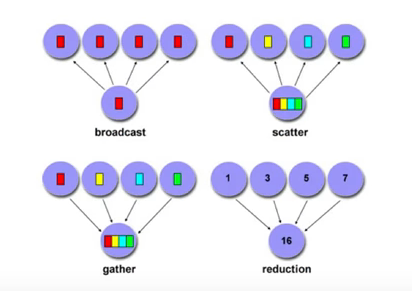
\includegraphics{Figures/mpi-diagram}
\decoRule
\caption[MPI Operations]{Four main supported MPI operations in mpi4py.}
\label{fig:MPI Operations}
\end{figure}


%----------------------------------------------------------------------------------------

\section{Docker}

Docker is an abstract, containerization system utilized for the automation and deployment of GNU/Linux operating systems.  Docker allows many single-images (known as containers) to run within one instance of Linux. This reduces the overhead of having to start and maintain many virtual machines.
    In the context of Docker, an image is a lightweight, executable package that has everything that is needed to run a piece of software, including code, libraries, environment variables, and configuration files. A container is the actual instance of an image when the image is executed on the operating system. The container runs independent of the host environment and can only access host files and networks if specified to do so. It is also important to note that containers run on the host machine’s kernel because the host kernel will produce better performance metrics than a virtual machine would. Figure 1.2 illustrates the aforementioned concepts.

\begin{figure}
\centering
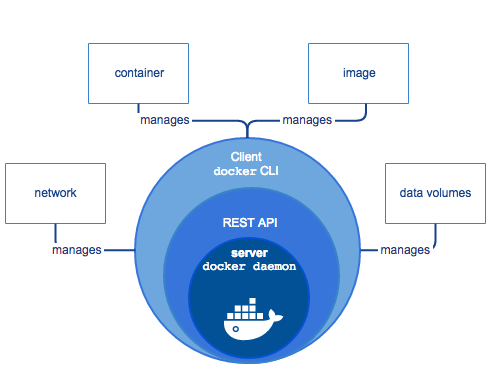
\includegraphics[scale=0.8]{Figures/docker-diagram}
\decoRule
\caption[Docker Architecture]{Illustration of Docker architecture.}
\label{fig:Docker Architecture}
\end{figure}


